\section{寄存器描述}
\regover{
{\hyperref[pwm-pwm-int-config]{pwm\_int\_config}}&
\\
\hline
{\hyperref[pwm-pwm-mc0-config0]{pwm\_mc0\_config0}}&
\\
\hline
{\hyperref[pwm-pwm-mc0-config1]{pwm\_mc0\_config1}}&
\\
\hline
{\hyperref[pwm-pwm-mc0-period]{pwm\_mc0\_period}}&
\\
\hline
{\hyperref[pwm-pwm-mc0-dead-time]{pwm\_mc0\_dead\_time}}&
\\
\hline
{\hyperref[pwm-pwm-mc0-ch0-thre]{pwm\_mc0\_ch0\_thre}}&
\\
\hline
{\hyperref[pwm-pwm-mc0-ch1-thre]{pwm\_mc0\_ch1\_thre}}&
\\
\hline
{\hyperref[pwm-pwm-mc0-ch2-thre]{pwm\_mc0\_ch2\_thre}}&
\\
\hline
{\hyperref[pwm-pwm-mc0-ch3-thre]{pwm\_mc0\_ch3\_thre}}&
\\
\hline
{\hyperref[pwm-pwm-mc0-int-sts]{pwm\_mc0\_int\_sts}}&
\\
\hline
{\hyperref[pwm-pwm-mc0-int-mask]{pwm\_mc0\_int\_mask}}&
\\
\hline
{\hyperref[pwm-pwm-mc0-int-clear]{pwm\_mc0\_int\_clear}}&
\\
\hline
{\hyperref[pwm-pwm-mc0-int-en]{pwm\_mc0\_int\_en}}&
\\
\hline
}

\subsection{pwm\_int\_config}
\label{pwm-pwm-int-config}
地址:0x4000a400
 \begin{figure}[H]
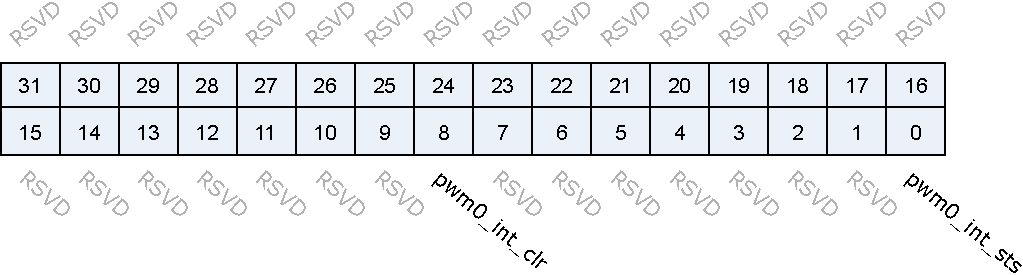
\includegraphics{pwm_pwm_int_config.pdf}
\end{figure}

\regdes{31:9&RSVD& & & \\\hline
8&pwm0\_int\_clr&w1c&1'b0&PWM 0 interrupt clear (clear pwm\_mc0\_int\_sts[10:0] all)\\\hline
7:1&RSVD& & & \\\hline
0&pwm0\_int\_sts&r&1'b0&PWM 0 interrupt status (Check pwm\_mc0\_int\_sts for detailed interrupt status)\\\hline

}
\subsection{pwm\_mc0\_config0}
\label{pwm-pwm-mc0-config0}
地址:0x4000a440
 \begin{figure}[H]
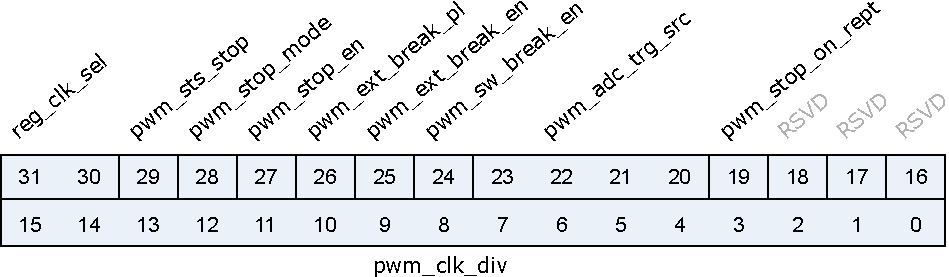
\includegraphics{pwm_pwm_mc0_config0.pdf}
\end{figure}

\regdes{31:30&reg\_clk\_sel&r/w&2'd0&PWM clock source select, 2'b00-xclk ; 2'b01-bclk ; others-f32k\_clk\\\hline
29&pwm\_sts\_stop&r&1'b0&PWM stop status\\\hline
28&pwm\_stop\_mode&r/w&1'b1&PWM stop mode, 1'b1 - graceful ; 1'b0 - abrupt\\\hline
27&pwm\_stop\_en&r/w&1'b0&PWM stop enable\\\hline
26&pwm\_ext\_break\_pl&r/w&1'b0&PWM external break source polarity \par 1'b0: Active-LOW \par 1'b1: Active-HIGH
\\\hline
25&pwm\_ext\_break\_en&r/w&1'b0&PWM external break source enable \par 1'b0: Disabled, external break signal is masked \par 1'b1: Enabled, external break signal is effective
\\\hline
24&pwm\_sw\_break\_en&r/w&1'b0&PWM break enable \par 1'b0: Disabled, normal operation \par 1'b1: Enabled, PWM output will be determined by CxPBS/CxNBS
\\\hline
23:20&pwm\_adc\_trg\_src&r/w&4'hF&Select signal of ADC triggering source \par 4'd0: pwm\_ch0l\_int (Channel 0 ThresholdL reached) \par 4'd1: pwm\_ch0h\_int (Channel 0 ThresholdH reached) \par 4'd2: pwm\_ch1l\_int (Channel 1 ThresholdL reached) \par 4'd3: pwm\_ch1h\_int (Channel 1 ThresholdH reached) \par 4'd4: pwm\_ch2l\_int (Channel 2 ThresholdL reached) \par 4'd5: pwm\_ch2h\_int (Channel 2 ThresholdH reached) \par 4'd6: pwm\_ch3l\_int (Channel 3 ThresholdL reached) \par 4'd7: pwm\_ch3h\_int (Channel 3 ThresholdH reached) \par 4'd8: pwm\_prde\_int (Period End reached) \par Others: Disabled
\\\hline
19&pwm\_stop\_on\_rept&r/w&1'b0&PWM stopped when rept\_int is asserted \par 1'b0: Disabled, PWM keeps running when rept\_int is asserted \par 1'b1: Enabled, PWM stops when rept\_int is asserted. Clear rept\_int to restore operation
\\\hline
18:16&RSVD& & & \\\hline
15:0&pwm\_clk\_div&r/w&16'b0&PWM clock division\\\hline

}
\subsection{pwm\_mc0\_config1}
\label{pwm-pwm-mc0-config1}
地址:0x4000a444
 \begin{figure}[H]
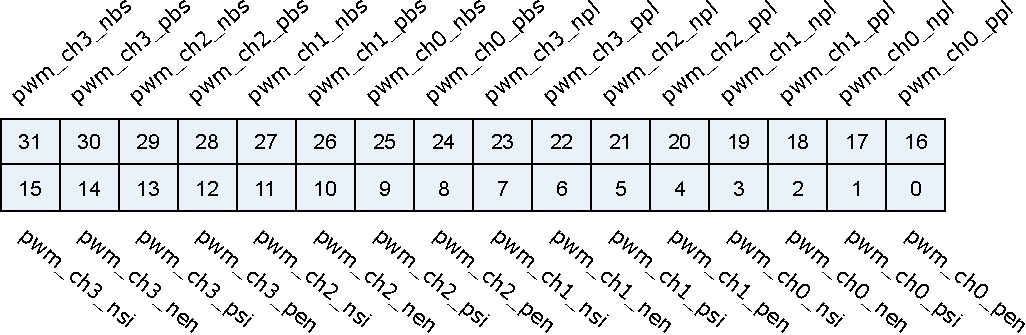
\includegraphics{pwm_pwm_mc0_config1.pdf}
\end{figure}

\regdes{31&pwm\_ch3\_nbs&r/w&1'b0&PWM channel 3 negative break state\\\hline
30&pwm\_ch3\_pbs&r/w&1'b0&PWM channel 3 positive break state\\\hline
29&pwm\_ch2\_nbs&r/w&1'b0&PWM channel 2 negative break state\\\hline
28&pwm\_ch2\_pbs&r/w&1'b0&PWM channel 2 positive break state\\\hline
27&pwm\_ch1\_nbs&r/w&1'b0&PWM channel 1 negative break state\\\hline
26&pwm\_ch1\_pbs&r/w&1'b0&PWM channel 1 positive break state\\\hline
25&pwm\_ch0\_nbs&r/w&1'b0&PWM channel 0 negative break state\\\hline
24&pwm\_ch0\_pbs&r/w&1'b0&PWM channel 0 positive break state\\\hline
23&pwm\_ch3\_npl&r/w&1'b1&PWM channel 3 negative polarity\\\hline
22&pwm\_ch3\_ppl&r/w&1'b1&PWM channel 3 positive polarity\\\hline
21&pwm\_ch2\_npl&r/w&1'b1&PWM channel 2 negative polarity\\\hline
20&pwm\_ch2\_ppl&r/w&1'b1&PWM channel 2 positive polarity\\\hline
19&pwm\_ch1\_npl&r/w&1'b1&PWM channel 1 negative polarity\\\hline
18&pwm\_ch1\_ppl&r/w&1'b1&PWM channel 1 positive polarity\\\hline
17&pwm\_ch0\_npl&r/w&1'b1&PWM channel 0 negative polarity\\\hline
16&pwm\_ch0\_ppl&r/w&1'b1&PWM channel 0 positive polarity\\\hline
15&pwm\_ch3\_nsi&r/w&1'b1&PWM channel 3 negative set idle state\\\hline
14&pwm\_ch3\_nen&r/w&1'b0&PWM channel 3 negative enable pwm out\\\hline
13&pwm\_ch3\_psi&r/w&1'b0&PWM channel 3 positive set idle state\\\hline
12&pwm\_ch3\_pen&r/w&1'b0&PWM channel 3 positive enable pwm out\\\hline
11&pwm\_ch2\_nsi&r/w&1'b1&PWM channel 2 negative set idle state\\\hline
10&pwm\_ch2\_nen&r/w&1'b0&PWM channel 2 negative enable pwm out\\\hline
9&pwm\_ch2\_psi&r/w&1'b0&PWM channel 2 positive set idle state\\\hline
8&pwm\_ch2\_pen&r/w&1'b0&PWM channel 2 positive enable pwm out\\\hline
7&pwm\_ch1\_nsi&r/w&1'b1&PWM channel 1 negative set idle state\\\hline
6&pwm\_ch1\_nen&r/w&1'b0&PWM channel 1 negative enable pwm out\\\hline
5&pwm\_ch1\_psi&r/w&1'b0&PWM channel 1 positive set idle state\\\hline
4&pwm\_ch1\_pen&r/w&1'b0&PWM channel 1 positive enable pwm out\\\hline
3&pwm\_ch0\_nsi&r/w&1'b1&PWM channel 0 negative set idle state\\\hline
2&pwm\_ch0\_nen&r/w&1'b0&PWM channel 0 negative enable pwm out\\\hline
1&pwm\_ch0\_psi&r/w&1'b0&PWM channel 0 positive set idle state\\\hline
0&pwm\_ch0\_pen&r/w&1'b0&PWM channel 0 positive enable pwm out\\\hline

}
\subsection{pwm\_mc0\_period}
\label{pwm-pwm-mc0-period}
地址:0x4000a448
 \begin{figure}[H]
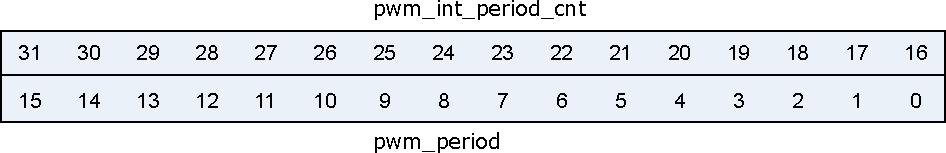
\includegraphics{pwm_pwm_mc0_period.pdf}
\end{figure}

\regdes{31:16&pwm\_int\_period\_cnt&r/w&16'd0&PWM interrupt period counter threshold\\\hline
15:0&pwm\_period&r/w&16'd0&PWM period setting\\\hline

}
\subsection{pwm\_mc0\_dead\_time}
\label{pwm-pwm-mc0-dead-time}
地址:0x4000a44c
 \begin{figure}[H]
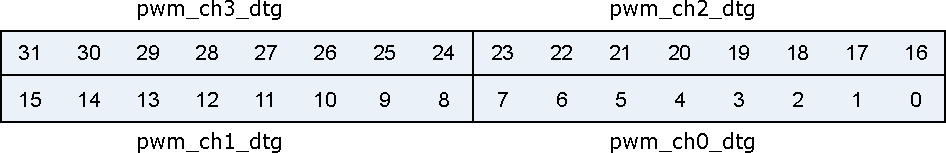
\includegraphics{pwm_pwm_mc0_dead_time.pdf}
\end{figure}

\regdes{31:24&pwm\_ch3\_dtg&r/w&8'h0&PWM Channel 3 dead time generator (DTG) \par DTG[7:5]=0xx => DT = DTG[7:0]*1 (unit: divided PWM clock) \par DTG[7:5]=10x => DT = (64+DTG[5:0])*2 (unit: divided PWM clock) \par DTG[7:5]=110 => DT = (32+DTG[4:0])*8 (unit: divided PWM clock) \par DTG[7:5]=111 => DT = (32+DTG[4:0])*16 (unit: divided PWM clock)
\\\hline
23:16&pwm\_ch2\_dtg&r/w&8'h0&PWM Channel 2 dead time generator (DTG) \par DTG[7:5]=0xx => DT = DTG[7:0]*1 (unit: divided PWM clock) \par DTG[7:5]=10x => DT = (64+DTG[5:0])*2 (unit: divided PWM clock) \par DTG[7:5]=110 => DT = (32+DTG[4:0])*8 (unit: divided PWM clock) \par DTG[7:5]=111 => DT = (32+DTG[4:0])*16 (unit: divided PWM clock)
\\\hline
15:8&pwm\_ch1\_dtg&r/w&8'h0&PWM Channel 1 dead time generator (DTG) \par DTG[7:5]=0xx => DT = DTG[7:0]*1 (unit: divided PWM clock) \par DTG[7:5]=10x => DT = (64+DTG[5:0])*2 (unit: divided PWM clock) \par DTG[7:5]=110 => DT = (32+DTG[4:0])*8 (unit: divided PWM clock) \par DTG[7:5]=111 => DT = (32+DTG[4:0])*16 (unit: divided PWM clock)
\\\hline
7:0&pwm\_ch0\_dtg&r/w&8'h0&PWM Channel 0 dead time generator (DTG) \par DTG[7:5]=0xx => DT = DTG[7:0]*1 (unit: divided PWM clock) \par DTG[7:5]=10x => DT = (64+DTG[5:0])*2 (unit: divided PWM clock) \par DTG[7:5]=110 => DT = (32+DTG[4:0])*8 (unit: divided PWM clock) \par DTG[7:5]=111 => DT = (32+DTG[4:0])*16 (unit: divided PWM clock)
\\\hline

}
\subsection{pwm\_mc0\_ch0\_thre}
\label{pwm-pwm-mc0-ch0-thre}
地址:0x4000a450
 \begin{figure}[H]
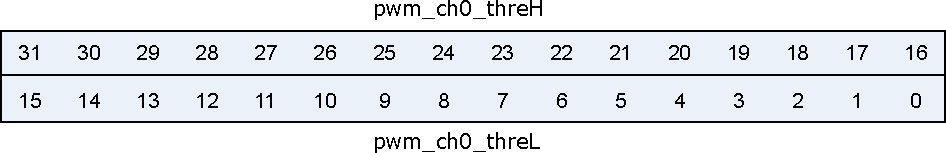
\includegraphics{pwm_pwm_mc0_ch0_thre.pdf}
\end{figure}

\regdes{31:16&pwm\_ch0\_threH&r/w&16'd0&PWM HIGH counter threshold, can't be smaller that threL\\\hline
15:0&pwm\_ch0\_threL&r/w&16'd0&PWM LOW counter threshold, can't be larger that threH\\\hline

}
\subsection{pwm\_mc0\_ch1\_thre}
\label{pwm-pwm-mc0-ch1-thre}
地址:0x4000a454
 \begin{figure}[H]
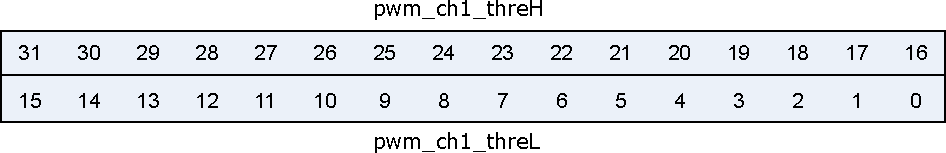
\includegraphics{pwm_pwm_mc0_ch1_thre.pdf}
\end{figure}

\regdes{31:16&pwm\_ch1\_threH&r/w&16'd0&PWM HIGH counter threshold, can't be smaller that threL\\\hline
15:0&pwm\_ch1\_threL&r/w&16'd0&PWM LOW counter threshold, can't be larger that threH\\\hline

}
\subsection{pwm\_mc0\_ch2\_thre}
\label{pwm-pwm-mc0-ch2-thre}
地址:0x4000a458
 \begin{figure}[H]
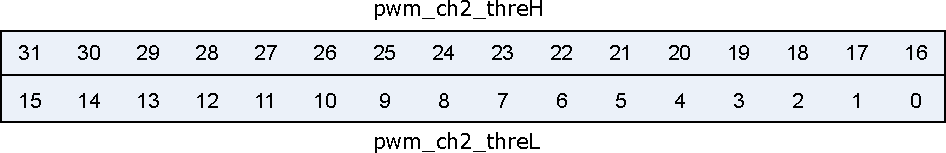
\includegraphics{pwm_pwm_mc0_ch2_thre.pdf}
\end{figure}

\regdes{31:16&pwm\_ch2\_threH&r/w&16'd0&PWM HIGH counter threshold, can't be smaller that threL\\\hline
15:0&pwm\_ch2\_threL&r/w&16'd0&PWM LOW counter threshold, can't be larger that threH\\\hline

}
\subsection{pwm\_mc0\_ch3\_thre}
\label{pwm-pwm-mc0-ch3-thre}
地址:0x4000a45c
 \begin{figure}[H]
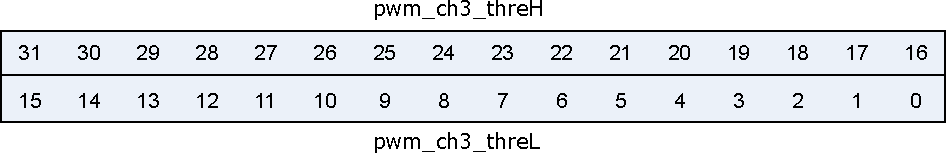
\includegraphics{pwm_pwm_mc0_ch3_thre.pdf}
\end{figure}

\regdes{31:16&pwm\_ch3\_threH&r/w&16'd0&PWM HIGH counter threshold, can't be smaller that threL\\\hline
15:0&pwm\_ch3\_threL&r/w&16'd0&PWM LOW counter threshold, can't be larger that threH\\\hline

}
\subsection{pwm\_mc0\_int\_sts}
\label{pwm-pwm-mc0-int-sts}
地址:0x4000a460
 \begin{figure}[H]
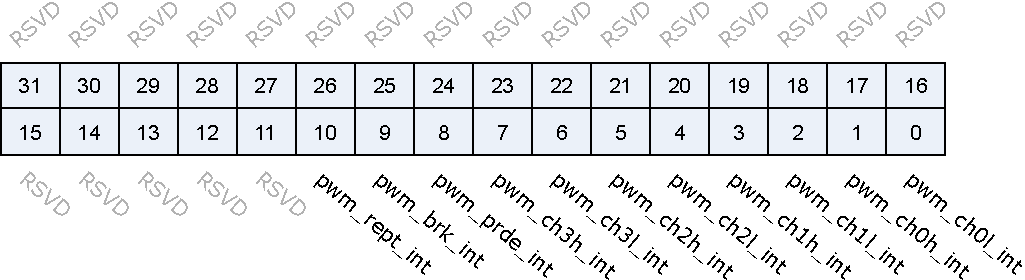
\includegraphics{pwm_pwm_mc0_int_sts.pdf}
\end{figure}

\regdes{31:11&RSVD& & & \\\hline
10&pwm\_rept\_int&r&1'b0&PWM repeat count interrupt status\\\hline
9&pwm\_brk\_int&r&1'b0&PWM break interrupt status, triggered when ext\_break is asserted \par Note: pwm\_sw\_break\_en will NOT trigger this interrupt
\\\hline
8&pwm\_prde\_int&r&1'b0&PWM period end interrupt status\\\hline
7&pwm\_ch3h\_int&r&1'b0&PWM Channel 3 ThresholdH interrupt status\\\hline
6&pwm\_ch3l\_int&r&1'b0&PWM Channel 3 ThresholdL interrupt status\\\hline
5&pwm\_ch2h\_int&r&1'b0&PWM Channel 2 ThresholdH interrupt status\\\hline
4&pwm\_ch2l\_int&r&1'b0&PWM Channel 2 ThresholdL interrupt status\\\hline
3&pwm\_ch1h\_int&r&1'b0&PWM Channel 1 ThresholdH interrupt status\\\hline
2&pwm\_ch1l\_int&r&1'b0&PWM Channel 1 ThresholdL interrupt status\\\hline
1&pwm\_ch0h\_int&r&1'b0&PWM Channel 0 ThresholdH interrupt status\\\hline
0&pwm\_ch0l\_int&r&1'b0&PWM Channel 0 ThresholdL interrupt status\\\hline

}
\subsection{pwm\_mc0\_int\_mask}
\label{pwm-pwm-mc0-int-mask}
地址:0x4000a464
 \begin{figure}[H]
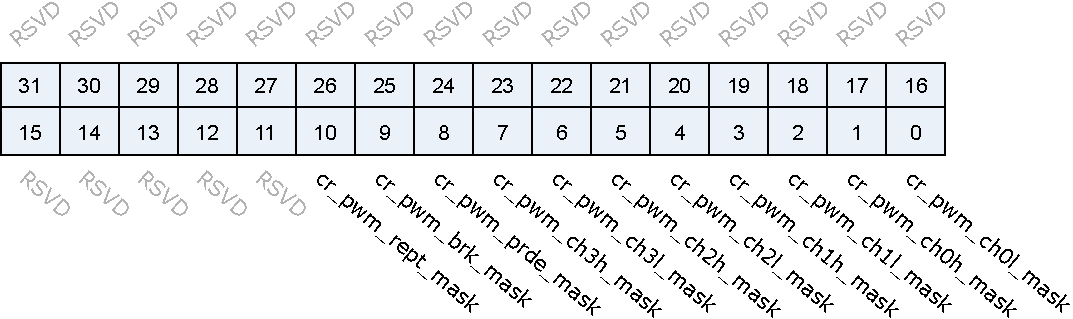
\includegraphics{pwm_pwm_mc0_int_mask.pdf}
\end{figure}

\regdes{31:11&RSVD& & & \\\hline
10&cr\_pwm\_rept\_mask&r/w&1'b1&Interrupt mask of pwm\_rept\_int\\\hline
9&cr\_pwm\_brk\_mask&r/w&1'b1&Interrupt mask of pwm\_brk\_int\\\hline
8&cr\_pwm\_prde\_mask&r/w&1'b1&Interrupt mask of pwm\_prde\_int\\\hline
7&cr\_pwm\_ch3h\_mask&r/w&1'b1&Interrupt mask of pwm\_ch3h\_int\\\hline
6&cr\_pwm\_ch3l\_mask&r/w&1'b1&Interrupt mask of pwm\_ch3l\_int\\\hline
5&cr\_pwm\_ch2h\_mask&r/w&1'b1&Interrupt mask of pwm\_ch2h\_int\\\hline
4&cr\_pwm\_ch2l\_mask&r/w&1'b1&Interrupt mask of pwm\_ch2l\_int\\\hline
3&cr\_pwm\_ch1h\_mask&r/w&1'b1&Interrupt mask of pwm\_ch1h\_int\\\hline
2&cr\_pwm\_ch1l\_mask&r/w&1'b1&Interrupt mask of pwm\_ch1l\_int\\\hline
1&cr\_pwm\_ch0h\_mask&r/w&1'b1&Interrupt mask of pwm\_ch0h\_int\\\hline
0&cr\_pwm\_ch0l\_mask&r/w&1'b1&Interrupt mask of pwm\_ch0l\_int\\\hline

}
\subsection{pwm\_mc0\_int\_clear}
\label{pwm-pwm-mc0-int-clear}
地址:0x4000a468
 \begin{figure}[H]
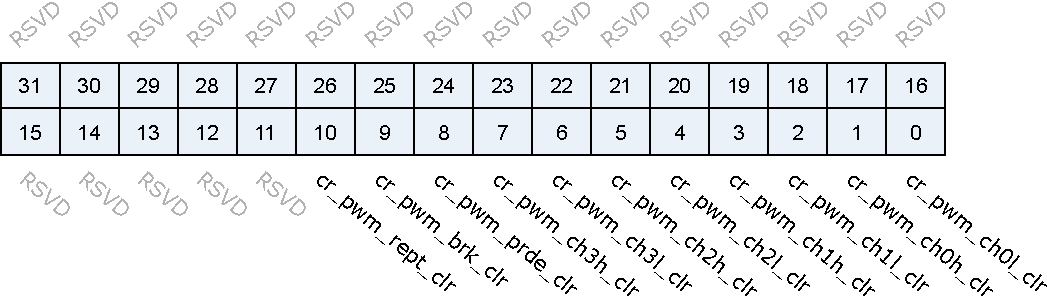
\includegraphics{pwm_pwm_mc0_int_clear.pdf}
\end{figure}

\regdes{31:11&RSVD& & & \\\hline
10&cr\_pwm\_rept\_clr&w1c&1'b0&Interrupt clear of pwm\_rept\_int\\\hline
9&cr\_pwm\_brk\_clr&w1c&1'b0&Interrupt clear of pwm\_brk\_int\\\hline
8&cr\_pwm\_prde\_clr&w1c&1'b0&Interrupt clear of pwm\_prde\_int\\\hline
7&cr\_pwm\_ch3h\_clr&w1c&1'b0&Interrupt clear of pwm\_ch3h\_int\\\hline
6&cr\_pwm\_ch3l\_clr&w1c&1'b0&Interrupt clear of pwm\_ch3l\_int\\\hline
5&cr\_pwm\_ch2h\_clr&w1c&1'b0&Interrupt clear of pwm\_ch2h\_int\\\hline
4&cr\_pwm\_ch2l\_clr&w1c&1'b0&Interrupt clear of pwm\_ch2l\_int\\\hline
3&cr\_pwm\_ch1h\_clr&w1c&1'b0&Interrupt clear of pwm\_ch1h\_int\\\hline
2&cr\_pwm\_ch1l\_clr&w1c&1'b0&Interrupt clear of pwm\_ch1l\_int\\\hline
1&cr\_pwm\_ch0h\_clr&w1c&1'b0&Interrupt clear of pwm\_ch0h\_int\\\hline
0&cr\_pwm\_ch0l\_clr&w1c&1'b0&Interrupt clear of pwm\_ch0l\_int\\\hline

}
\subsection{pwm\_mc0\_int\_en}
\label{pwm-pwm-mc0-int-en}
地址:0x4000a46c
 \begin{figure}[H]
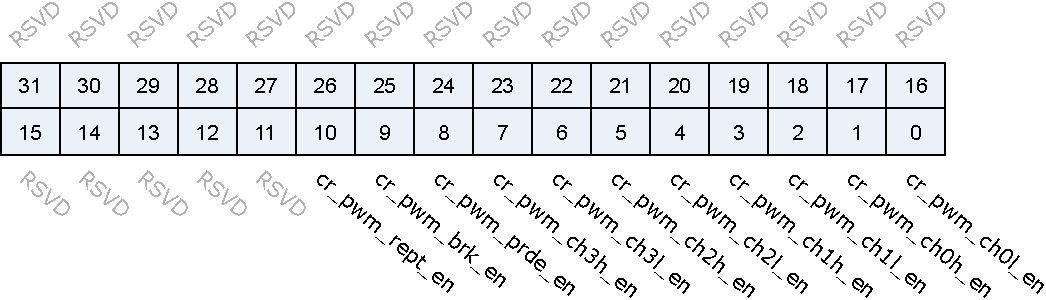
\includegraphics{pwm_pwm_mc0_int_en.pdf}
\end{figure}

\regdes{31:11&RSVD& & & \\\hline
10&cr\_pwm\_rept\_en&r/w&1'b1&Interrupt enable of pwm\_rept\_int\\\hline
9&cr\_pwm\_brk\_en&r/w&1'b1&Interrupt enable of pwm\_brk\_int\\\hline
8&cr\_pwm\_prde\_en&r/w&1'b1&Interrupt enable of pwm\_prde\_int\\\hline
7&cr\_pwm\_ch3h\_en&r/w&1'b1&Interrupt enable of pwm\_ch3h\_int\\\hline
6&cr\_pwm\_ch3l\_en&r/w&1'b1&Interrupt enable of pwm\_ch3l\_int\\\hline
5&cr\_pwm\_ch2h\_en&r/w&1'b1&Interrupt enable of pwm\_ch2h\_int\\\hline
4&cr\_pwm\_ch2l\_en&r/w&1'b1&Interrupt enable of pwm\_ch2l\_int\\\hline
3&cr\_pwm\_ch1h\_en&r/w&1'b1&Interrupt enable of pwm\_ch1h\_int\\\hline
2&cr\_pwm\_ch1l\_en&r/w&1'b1&Interrupt enable of pwm\_ch1l\_int\\\hline
1&cr\_pwm\_ch0h\_en&r/w&1'b1&Interrupt enable of pwm\_ch0h\_int\\\hline
0&cr\_pwm\_ch0l\_en&r/w&1'b1&Interrupt enable of pwm\_ch0l\_int\\\hline

}
